%28/01 - Aythami Morales 
\chapter{Introducción}
%\section{Review: Álgebra lineal}

\section{Introducción al Aprendizaje Automático o Machine Learning}
\subsection{Contexto histórico}
Hay muchas definiciones de aprendizaje automático. Según Wikipedia, machine learning es la construcción y estudio de sistemas que pueden aprender de datos. Arthur Samuel lo definía como un campo de estudio que confiere a los ordenadores la capacidad de aprender sin ser programados explícitamente. En el aprendizaje automático, no se diseña el algoritmo para que resuelva una tarea con unas reglas fijas, si no para que con una serie de datos pueda aprender a resolver la tarea. 

Arthur Samuel, en la década de 1950, escribió un programa para jugar a las damas que era capaz de aprender las mejores posiciones del tablero analizando miles de partidas. El sistema aprendió por sí mismo a jugar a las damas cada vez mejor. El 11 de mayo de 1997, el gran maestro de ajedrez Garry Kasparov renuncia tras 19 movimientos en una partida contra Deep Blue, un ordenador ajedrecista desarrollado por científicos de IBM. En 2016, Google (AlphaGo) derrotó al campeón mundial de Go. Este juego fue considerado durante décadas uno de los grandes retos de la IA. \footnote{Para el ajedrez, no se trata realmente de una inteligencia artificial, si no una máquina que calcula probabilidades. Cada movimiento proporciona una probabilidad de vencer al contrincante. Hay aperturas del ajedrez que facilitan un poco la victoria. Esto para el Go no existe. La máquina pudo encontrar una táctica para el Go nunca antes descrita, abriendo el debate de si se trata de creatividad.} En 2020, Google (AlphaFold) predice la estructura de las proteínas. Aquí se basa de \textbf{aprendizaje por refuerzo}. Se utilizó AlphaGo como base para generar otros modelos similares: AlphaChess, AlphaFold, etc. Las damas, el ajedrez, el go y las estructuras de las proteínas tienen en común ser problemas con unas reglas bien definidas. A partir de reglas sencillas, se generan estructuras complejas. Por ello, son campos donde se puede predecir o estimar muchas combinaciones y posibles variaciones. Estos algoritmos funcionan por prueba y error, por lo que no tiene sentido aplicarlo en otros campos donde los errores tienen consecuencias graves, como puede ser el diagnóstico de enfermedades o la conducción autónoma de coches. En general, todo el comportamiento humano es imposible de describir en reglas; cada paciente es muy complejo en sí mismo, siendo difícil generalizar en poblaciones grandes por procesos moleculares, comportamiento, epigenética, etc. 

La IA se ha democratizado mucho con los softwares open-source. Tecnológicamente no hay secretos a día de hoy, solo diferencias en los datos y el hardware. 

\subsection{De programación clásica al aprendizaje automático}
Los humanos adquieren con el tiempo experiencias que les hace aprender, causando respuestas concretas a distintas situaciones. Los ordenadores y las máquinas obtienen reglas predefinidas y datos, y con programación clásica llegan a su respuesta. No obstante, actualmente se utilizan datos y respuestas para, mediante aprendizaje automático, poder inferir las reglas. Esto invierte la forma de funcionar los ordenadores, y ha sido lo revolucionario del campo. Esas reglas inferidas se utilizarán para nuevos datos y poder ser cada vez más precisas. Así, el algoritmo encuentra las mejores reglas para resolver un problema. Estas reglas son ecuaciones matemáticas, pudiendo ser propensas a sesgos en base a los datos.

\subsection{De comportamiento humano a comportamiento computacional: el modelo estándar}
Una tarea humana se realiza a través de unos objetivos mediante abstracción. El proceso de aprendizaje está guiado por objetivos predefinidos (es decir, la simplificación de comportamientos complejos). En el caso de las máquinas,  el proceso de aprendizaje consta de etapas de optimización para llegar al objetivo. Al final se trata de una reducción y optimización de la abstracción humana. No obstante, no hay una visión directa entre el comportamiento de la máquina y el comportamiento humano. No se puede esperar que un algoritmo sea justo o generoso por naturaleza si no se especifica en sus objetivos. Por ello, es muy fácil que aparezcan sesgos en el aprendizaje automático. La toma de decisión es muy diferente entre un humano y una máquina.

\subsection{Cómo ve la IA: Un ejemplo con ataques adversarios}
Tenemos una imagen de un cerdo (figura \ref{fig:pig}), y no necesitamos el ruido para saber lo que es. Si le añadimos ruido a la imagen, aunque sea en una baja cantidad, la imagen no cambia para los humanos. No obstante, el sistema de reconocimiento de imágenes lo reconoce como una aerolínea. El ruido no es aleatorio, si no adversario. Esto quiere decir que la entrada al modelo ha sido modificada ligeramente de forma intencional, haciendo que el modelo genere una salida incorrecta. Se manipula para confundir a la máquina.

\begin{figure}[htbp]
\centering
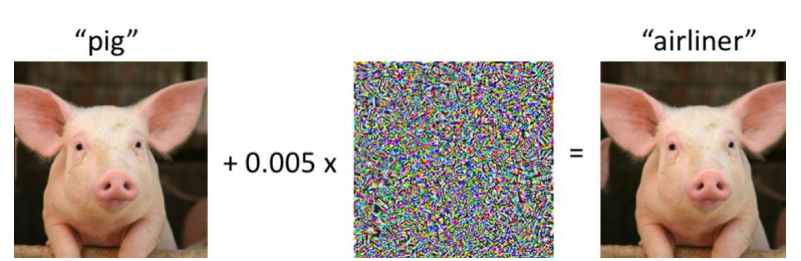
\includegraphics[width = 0.9\textwidth]{figs/pig-ai.png}
\caption{Reconocimiento de imágenes con ataque adversario.}
\label{fig:pig}
\end{figure}

\subsection{Cognición humana: sistema 1 vs sistema 2}
Los conceptos del libro Thinking, Fast and Slow de Daniel Kahneman se han aplicado en el campo del aprendizaje automático. Se habla de dos sistemas y categorías de tareas cognitivas. El \textbf{sistema 1} es intuitivo, rápido, inconsciente, no lingüístico y habitual. Se decía que el aprendizaje profundo estaba en ese sistema. El \textbf{sistema 2} es lento, lógico, secuencial, consciente, lingüístico, algorítmico, y es donde estaría el deep learning futuro. Esto sirvió para el aprendizaje automático de estructuras de datos: redes de cápsulas, aprendizaje automático neurosintáctico, razonamiento conceptual, bases de experiencia, reglas lógicas, etc. \textit{El sistema 1 sirve para reconocer formas, colores y posiciones, mientras que el sistema 2 ayuda en la predicción de interacciones.}

\subsection{Tarea de aprendizaje}
Se dice que un programa informático aprende de la experiencia E con respecto a alguna tarea T y alguna medida de rendimiento P, si su rendimiento en T, medido por P, mejora con la experiencia E. Si el rendimiento es perfecto desde el principio, no hay aprendizaje, ya que requiere una optimización o mejora del estado. Ejemplos son:
\begin{itemize}
\item T: Jugar a las damas \\ P: Porcentaje de partidas ganadas contra un contrincante arbitrario \\ E: Jugar partidas de práctica contra uno mismo
\item T: Reconocer palabras escritas a mano \\ P: Porcentaje de palabras clasificadas correctamente \\ E: Base de datos de imágenes de palabras manuscritas etiquetadas por humanos
\item T: Conducción en autopistas de cuatro carriles mediante sensores de visión \\ P: Distancia media recorrida antes de un error apreciado por el ser humano \\ E: Secuencia de imágenes y comandos de dirección grabados mientras se observa a un conductor humano.
\item T: clasificar los mensajes de correo electrónico como spam o legítimos. \\ P: Porcentaje de mensajes de correo electrónico clasificados correctamente. \\ E: Base de datos de correos electrónicos, algunos con etiquetas dadas por humanos.
\end{itemize}

\subsection{Aprendizaje automático en contexto}
En el núcleo de la IA, el aprendizaje automático es simplemente una forma de conseguir IA. En lugar de codificar rutinas de software con instrucciones específicas para realizar una tarea concreta, el ML es una forma de «entrenar» un algoritmo para que aprenda a hacerlo. El «entrenamiento» consiste en introducir grandes cantidades de datos en el algoritmo y permitir que éste se ajuste y mejore.

\begin{figure}[htbp]
\centering
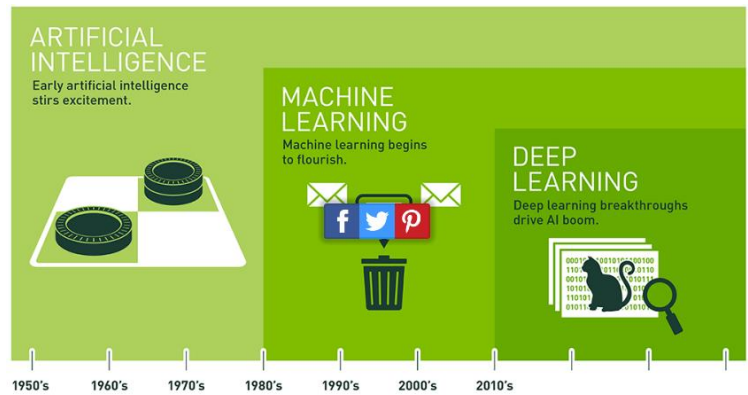
\includegraphics[width = 0.8\textwidth]{figs/ai-timeline.png}
\caption{Mapa temporal del desarrollo de las inteligencias artificiales. Ya está algo desfasado, faltaría añadir después del Deep Learning los Modelos Generativos.}
\end{figure}

No se trata de comparar el aprendizaje humano vs aprendizaje automático, si no combinar ambos para sacar lo mejor de los dos mundos. Habrá tareas que se irán automatizando.

\subsection{Diseño de sistema de aprendizaje}
Muchos métodos de aprendizaje implican formación. La formación es la adquisición de conocimientos, destrezas y competencias como resultado de la enseñanza de aptitudes o conocimientos prácticos relacionados con una competencia útil. La formación requiere escenarios o ejemplos (datos). Existen varios tipos de sistemas de aprendizaje:
\begin{itemize}
\item \textbf{No supervisado:} sin respuestas o comentarios/feedback.
\item \textbf{Supervisado:} utiliza una serie de ejemplos etiquetados con retroalimentación directa.
\item \textbf{Aprendizaje de refuerzo:} retroalimentación indirecta, después de muchos ejemplos.
\end{itemize}

\subsubsection{Supervisado vs no supervisado}
Supongamos una función desconocida $y_{\Theta}(\mathrm{\textbf{x}}) = h_{\Theta}(\mathrm{\textbf{x}})$, donde x es un ejemplo de entrada y y la salida deseada. El \textbf{aprendizaje supervisado} implica que recibimos un conjunto de pares de entrenamiento (x,y) por un "profesor". De esta forma, se puede entender la generación de h para cuando se obtenga solo la salida en una prueba, sin conocer la salida de antemano. En el caso del \textbf{aprendizaje no supervisado}, sólo se nos da la $\mathrm{\textbf{x}}$ y alguna función (última) de retroalimentación sobre nuestro rendimiento. $\Theta$ hace referencia a los parámetros que tiene el modelo y que hay que entrenar. Por tanto, cuantos menos parámetros haya, más rápido va a ser el modelo.

Las fases de un algoritmo de aprendizaje son:
\begin{enumerate}
\item \textbf{Hipótesis, datos}

Los datos son $\mathrm{\textbf{x}}_n = (x_{n1} ... x_{nD})^T$ y las etiquetas $y_n$ como salida deseada (solo en el caso del aprendizaje supervisado). Los datos pueden ser numéricos, categóricos, texto o series temporales. Aunque no haya una notación general, vamos a utilizar la negrita no itálica para denominar que la variable es un vector. D define la dimensión del vector, y el superíndice T hace referencia a la naturaleza del vector (es un trauma matemático). La información puede estar estructurada (datos genéticos, metereológicos, etc) o no estructurada (imágenes, audio, texto).

\item \textbf{Selección del modelo}

Hay que seleccionar el modelo $h_{\Theta}(\mathrm{\textbf{x}})$: 
$$y(\mathrm{\textbf{x}}) = h(\mathrm{\textbf{x}}) \rightarrow y_{\Theta}(\mathrm{\textbf{x}}) = h_{\Theta}(\mathrm{\textbf{x}}) = h(\mathrm{\textbf{x}}) + \epsilon$$

\begin{figure}[h]
\centering
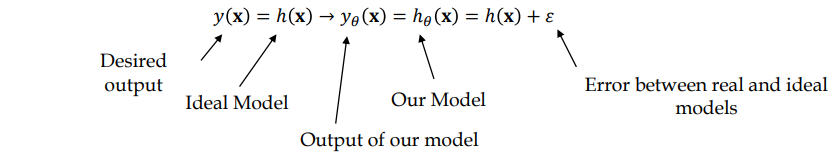
\includegraphics[width = \textwidth]{figs/model-htheta.png}
\end{figure}

Por ejemplo, si queremos modelar una recta $h_{\Theta}(\mathrm{\textbf{x}}) = a\mathrm{\textbf{x}} + b$, $a$ se correspondería a $\Theta_1$ y $b$ a $\Theta_2$. Encontrar $a$ y $b$ óptimos es imprescindible para un buen ajuste. Se debe seleccionar la métrica P a través de la que mejorar el aprendizaje. Así, la función del coste se resume en:
$$E(y_{\Theta} - y)^2 = [h_{\Theta}(\mathrm{\textbf{x}}) - h(\mathrm{\textbf{x}})]^2 + \epsilon$$

siendo $ [h_{\Theta}(\mathrm{\textbf{x}}) - h(\mathrm{\textbf{x}})]^2$ el coste reducible y $\epsilon$ el irreducible. El reducible se puede mejorar mediante la optimización de los parámetros, mientras que la irreducible cambiando el modelo/hipótesis.

\item \textbf{Entrenamiento o aprendizaje}
\item \textbf{Testeo o inferencia}
\end{enumerate}

%\section{Reducción de dimensionalidad}
